\documentclass{article}
\usepackage[utf8]{inputenc}
\usepackage{multicol}
\usepackage{graphicx}
\usepackage{geometry}
\usepackage{color}
\usepackage{amssymb}
\usepackage{graphicx}
\usepackage{caption}
\usepackage{subcaption}


\begin{document}


\section{Genetic Algorithm (GA)}


% Reference Holland (inventor)
% Reference Darwin (evolution)
% Reference Goldberg (description)


% Why GA
Genetic algorithms are probabilistic search algorithms inspired by natural selection and survival of the fittest. They operate on complex problems that would be very difficult, maybe even impossible, to solve by classical methods. Genetic algorithms are very robust and can find near-optimal solutions to problems without knowing anything about how an optimal solution look like, they only require a method of measuring the "goodness" or fitness of a solution.


% How GA works
Genetic algorithms work as follows: An initial population of individual solutions is generated and the fitness of each individual is calculated based on a fitness function, which from now on will be called an objective function. Based on their objective function values the fittest individuals are selected for reproduction. By combining genes of the parent solutions and perform genetic operations such as mutation, a new pool of solutions is generated. Since the solutions of the newly generated population is produced by recombining the fittest solutions from the initial population the average fitness of the newly generated population is expected to be higher than the one of the initial population. This process continues until some stopping condition is reach, and by then the average and best fitness of the population should be pretty high. Figure \ref{GA Flow chart} shows the main operations of the genetic algorithm.


% Figure of GA
\begin{figure}[h!]
\begin{center}
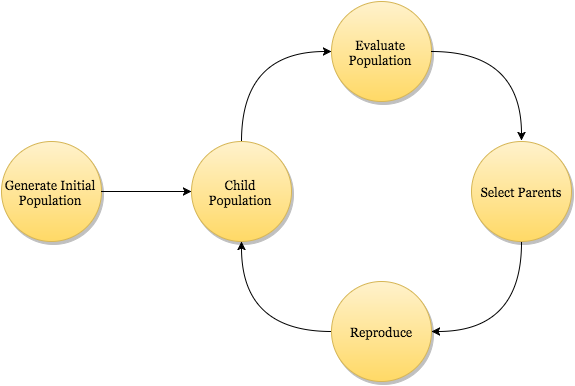
\includegraphics[scale=0.5]{GA}
\caption{The main operations of and genetic algorithm}
\end{center}
\label{GA Flow chart}
\end{figure}


% Representation
%\subsubsection{Representation of individuals and Reproduction}
%The individuals (solutions) that the GA perform operations on are represented as bit-strings. Initially each bit-string is generated by randomly assigning either zero or one to each of the ''genes'' of the individual. An example of an individual is given below:
%
%
%\begin{figure}[h!]
%    \centering
%    \begin{subfigure}[b]{0.3\textwidth}
%        \includegraphics[width=\textwidth]{"Single Point Crossover"}
%        \caption{Single-point crossover.}
%        \label{fig:gull}
%    \end{subfigure}
%    ~ %add desired spacing between images, e. g. ~, \quad, \qquad, \hfill etc. 
%      %(or a blank line to force the subfigure onto a new line)
%    \begin{subfigure}[b]{0.3\textwidth}
%        \includegraphics[width=\textwidth]{"Double Point Crossover"}
%        \caption{Double-point crossover.}
%        \label{fig:tiger}
%    \end{subfigure}
%    \caption{Crossover operations. (a) Singe point crossover at position four. (b) Double-point crossover at positions three and nine.}\label{fig:animals}
%\end{figure}


\subsection{The Island Model}
The island model is an extension of the general GA where the initial population of size $N_{total}$ is partitioned into $N_{island}$ such that each island holds a population of size $N_{total} / N_{island}$. The separated populations can then evolve on each island, exploring different solutions, until a migration takes place. A migration is when some individuals from one island migrate to another island. Figure \ref{Island Model} shows an island model consisting of four island where the arrows shows legal migration routes. The topology of the island network and migration routes can take many different forms. 

The advantage of using the island model, as compared to the classical GA is that in the classical GA the population can converge to a non-optimal solution quite fast, because a few individuals can take over the entire population and guide it towards a sub-optimal solution. Using the island model the probability of converging to a sub-optimal solution will decrease because each island can investigate a different part of the solution space. 


\begin{figure}[h!]
\begin{center}
\includegraphics[scale=0.5]{"Island Model"}
\caption{Island Model}
\end{center}
\label{Island Model}
\end{figure}


\subsection{The Cellular Model}


\begin{figure}[h!]
\begin{center}
\includegraphics[scale=0.5]{"Cellular Model"}
\caption{Cellular Model}
\end{center}
\label{Cellular Model}
\end{figure}


\end{document}